\documentclass[tikz,border=12pt]{standalone}
\usepackage[T1]{fontenc}
\usetikzlibrary{positioning}
\begin{document}
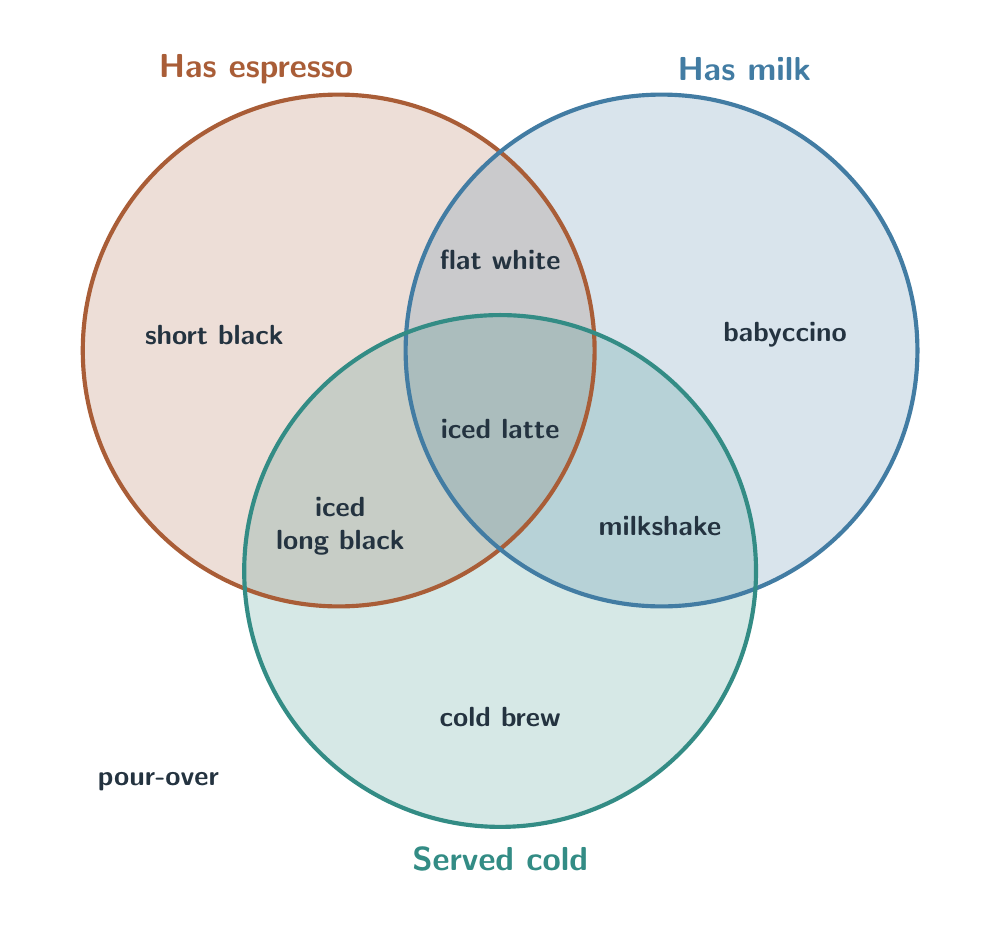
\begin{tikzpicture}[font=\sffamily]
  % Three independent properties: overlapping transparent disks make all
  % seven interior regions visible without hiding their boundaries.
  \definecolor{espresso}{HTML}{A95D37}
  \definecolor{milk}{HTML}{427CA3}
  \definecolor{cold}{HTML}{338C85}
  \definecolor{ink}{HTML}{243340}
  \fill[white] (-6.0,-5.85) rectangle (6.0,5.25);
  \fill[espresso,opacity=.20] (-2.05,1.15) circle (3.25);
  \fill[milk,opacity=.20] (2.05,1.15) circle (3.25);
  \fill[cold,opacity=.20] (0,-1.65) circle (3.25);
  \draw[espresso,line width=1.5pt] (-2.05,1.15) circle (3.25);
  \draw[milk,line width=1.5pt] (2.05,1.15) circle (3.25);
  \draw[cold,line width=1.5pt] (0,-1.65) circle (3.25);

  \tikzset{drink/.style={text=ink,align=center,font=\sffamily\bfseries\normalsize,inner sep=2pt},
            property/.style={font=\sffamily\bfseries\large,inner sep=3pt}}
  \node[property,text=espresso] at (-3.10,4.72) {Has espresso};
  \node[property,text=milk] at (3.10,4.72) {Has milk};
  \node[property,text=cold] at (0,-5.31) {Served cold};

  \node[drink] at (-3.63,1.35) {short black};
  \node[drink] at (3.62,1.35) {babyccino};
  \node[drink] at (0,2.30) {flat white};
  \node[drink] at (-2.03,-1.08) {iced\\long black};
  \node[drink] at (2.03,-1.08) {milkshake};
  \node[drink] at (0,0.16) {iced latte};
  \node[drink] at (0,-3.50) {cold brew};
  \node[drink] at (-4.34,-4.33) {pour-over};
\end{tikzpicture}
\end{document}
